%%%%%%%%%%%%%%%%%%%%%%%%%%%%%%%%%%%%%%%%%%%%%%%%%%%%%%%%%%%%%%%%%%%%%%
% Lớp 10 | Véctơ (chưa xét tọa độ) | Tích của một số với véctơ
% Dạng 0H5?3-4: Sự cùng phương của 2 véctơ và ứng dụng
% Số câu: 3  (sinh tự động bởi tach_cau.py; từ nay thầy sửa trực tiếp file này)
%%%%%%%%%%%%%%%%%%%%%%%%%%%%%%%%%%%%%%%%%%%%%%%%%%%%%%%%%%%%%%%%%%%%%%

%%%%%%%%%%%%%%%% TRẮC NGHIỆM 4 PHƯƠNG ÁN %%%%%%%%%%%%%%%%

% nguồn: MaHoaNH_TracNghiem_Lop10
\begin{ex}%[0H5N3-4]%[ma:86c90061]
	Cho ba điểm $A$, $B$, $C$ phân biệt. Điều kiện cần và đủ để ba điểm $A$, $B$, $C$ thẳng  hàng là
	\choice 
		{$AB=AC$} 
		{\True $\exists k\ne 0$ sao  cho $\overrightarrow{AB}=k\cdot \overrightarrow{AC}$}
		{$\overrightarrow{AC}-\overrightarrow{AB}=\overrightarrow{BC}$} 
		{$\overrightarrow{MA}+\overrightarrow{MB}=3\overrightarrow{MC}$ với mọi  điểm $M$}
	\loigiai{ 
		Điều kiện cần và đủ để ba điểm $A$, $B$, $C$ thẳng hàng là $\exists k\ne 0$  sao cho $\overrightarrow{AB}=k\cdot \overrightarrow{AC}$.
	} 
\end{ex}


%%%%%%%%%%%%%%%% ĐÚNG/SAI %%%%%%%%%%%%%%%%

% nguồn: MaHoaNH_DungSai_Lop10
\begin{ex}%[0H5N3-4]%[ma:6b879a7d]
	Cho hình chữ nhật  $ABCD$ có $O$ là giao điểm của hai đường chéo. Xét tính đúng sai của các mệnh đề sau
	 \choiceTF
		{\True $\overrightarrow{AB}$  và $\overrightarrow{CD}$ cùng phương}
		{\True  $\overrightarrow{AB}$ và $\overrightarrow{DC}$ cùng hướng}
		{\True $\overrightarrow{AO}$  và $\overrightarrow{CO}$ cùng phương}
		{\True  $\overrightarrow{AD}$ và $\overrightarrow{DA}$ ngược hướng}
	\loigiai{ 
		\begin{itemchoice}
			\itemch Vì $ABCD$ là hình bình hành nên $\overrightarrow{AB}$ và  $\overrightarrow{CD}$ cùng phương.
			\itemch Vì $ABCD$ là hình  bình hành nên $\overrightarrow{AB}$ và $\overrightarrow{DC}$ cùng hướng.
			\itemch Hai  véc-tơ $\overrightarrow{AO}$ và $\overrightarrow{CO}$ cùng phương vì có giá trùng nhau.
			\itemch Hai véc-tơ $\overrightarrow{AD}$ và  $\overrightarrow{DA}$ ngược hướng vì $\overrightarrow{AD}=-\overrightarrow{DA}$.
		\end{itemchoice}
	 }
\end{ex}

% nguồn: MaHoaNH_DungSai_Lop10
\begin{ex}%[0H5N3-4]%[ma:ee03775e]
	Cho tam giác $ABC$. Đặt $\vec{a}=\overrightarrow{BC};\, \vec{b}=\overrightarrow{AC}$.  Xét tính đúng sai của các mệnh đề sau. Các cặp véc-tơ
	 \choiceTF
		{$2\vec{a}+\vec{b}$ và  $\vec{a}+2\vec{b}$ cùng phương}
		{$\vec{a}-2\vec{b}$  và $2\vec{a}-\vec{b}$ cùng phương}
		{\True $5\vec{a}+\vec{b}$ và $-10\vec{a}-2\vec{b}$ cùng  phương}
		{\True $\vec{a}+\vec{b}$  và $-\vec{a}-\vec{b}$ cùng phương}
	\loigiai{ 
		\begin{itemchoice}
			\itemch Hai véc-tơ $2\vec{a}+\vec{b}$  và $\vec{a}+2\vec{b}$ không cùng phương.
			\itemch Hai  véc-tơ $\vec{a}-2\vec{b}$ và $2\vec{a}-\vec{b}$ không cùng phương.
			\itemch Vì  $-10\vec{a}-2\vec{b} = -2(5\vec{a}+\vec{b})$ nên hai véc-tơ $5\vec{a}+\vec{b}$ và $-10\vec{a}-2\vec{b}$ cùng phương.
			\itemch Vì $-\vec{a}-\vec{b}=(-1)\cdot(\vec{a}+\vec{b})$ nên hai véc-tơ  $\vec{a}+\vec{b}$ và $ -\vec{a}-\vec{b}$ cùng phương.
		\end{itemchoice}
	 }
\end{ex}

% nguồn: TuLuan_Lop10_daduyet (nhập 14/11/2026)
\begin{bt}%[0H5C3-4]%[Dự án đề kiểm tra Toán 10 HKI NH24-25- Lê Minh Thiện Anh]%[TH-THCS-THPT Hoang Viet- Đắk Lắk]%[ma:3b1485c0]
	Cho tam giác $ABC$ có $I$ là trung điểm của $BC$. Điểm $M$ là điểm thỏa mãn $\overrightarrow{MA}+\overrightarrow{MI}=\overrightarrow{0}$. Điểm $N$ thuộc cạnh $AC$ thỏa $AC=3CN$, điểm $E$ là giao điểm của đường thẳng $MN$ và đường thẳng $AB$. Tính tỉ số $\dfrac{AE}{AB}$.
	\loigiai{
		\begin{center}
		\begin{tikzpicture}[>=stealth,line join=round,line cap=round,font=\footnotesize,scale=1]
				\path (2,3) coordinate (A)
				(0,0) coordinate (B)
				(6,0) coordinate (C)
				($(B)!1/2!(C)$) coordinate (I)
				($(A)!1/2!(I)$) coordinate (M)
				($(A)!2/3!(C)$) coordinate (N)
				(intersection of A--B and M--N) coordinate (E)
				; 
				\draw (A)--(B)--(C)--(A) (A)--(I) (N)--(E)
				;
				\foreach \p/\r in {A/90,B/180,C/0,I/-90,N/60,E/190,M/60}
				\fill (\p) circle (1pt) node[shift={(\r:3mm)}]{$\p$};
				\end{tikzpicture}		
		\end{center}	 
		Vì $\overrightarrow{MA}+\overrightarrow{MI}=\overrightarrow{0}$ nên $M$ là trung điểm của $AI$.\\
		Đặt $k=\dfrac{AE}{AB}\Rightarrow \overrightarrow{AE}=k\cdot\overrightarrow{AB}$
		$AC=3CN\Rightarrow \overrightarrow{AN}=\dfrac{2}{3}\overrightarrow{AC}$.\\
		Ta có $\overrightarrow{EN}=\overrightarrow{AN}-\overrightarrow{AE}=-k\cdot\overrightarrow{AB}+\dfrac{2}{3}\overrightarrow{AC}$.\quad $(1)$\\
		Mặt khác $\overrightarrow{MN}=\overrightarrow{AN}-\overrightarrow{AM}=\overrightarrow{AN}-\dfrac{1}{2}\overrightarrow{AI}=\dfrac{2}{3}\overrightarrow{AC}-\dfrac{1}{4}\left( \overrightarrow{AB}+\overrightarrow{AC} \right)=-\dfrac{1}{4}\overrightarrow{AB}+\dfrac{5}{12}\overrightarrow{AC}$. \quad $(2)$\\
		Vì $M$, $N$, $E$ thẳng hàng nên từ $(1)$, $(2)$ suy ra $\dfrac{-k}{-\tfrac{1}{4}}=\dfrac{\tfrac{2}{3}}{\tfrac{5}{12}}\Leftrightarrow 4k=\dfrac{8}{5}\Rightarrow k=\dfrac{2}{5}$.\\
		Vậy $\dfrac{AE}{AB}=\dfrac{2}{5}$.		
	}
\end{bt}

% nguồn: TuLuan_Lop10_Dot2 (nhập 14/11/2026)
\begin{bt}%[0H5V3-4]%[ma:7ec274fd]
	Cho tam giác $ABC$ có trung tuyến $AM$. Gọi $I$ là trung điểm $AM$ và $K$ là  điểm thuộc $AC$ sao $AK=\dfrac{1}{3}AC$. Chứng minh ba điểm $B, I, K$ thẳng hàng.
	\loigiai{
		\immini
		{
			Ta có $2\overrightarrow{BI}=\overrightarrow{BA}+\overrightarrow{BM}=\overrightarrow{BA}+\dfrac{1}{2}\overrightarrow{BC}$ \\
			$\Rightarrow 4\overrightarrow{BI}=2\overrightarrow{BA}+\overrightarrow{BC}.\quad(1)$\\
			Ta có
			\allowdisplaybreaks
			\begin{eqnarray*}
				\overrightarrow{BK}&=&\overrightarrow{BA}+\overrightarrow{AK} \\
				&=&\overrightarrow{BA}+\dfrac{1}{3}\overrightarrow{AC} \\ &=&\overrightarrow{BA}+\dfrac{1}{3}(\overrightarrow{BC}-\overrightarrow{BA}) \\
				&=&\dfrac{2}{3}\overrightarrow{BA}+\dfrac{1}{3}\overrightarrow{BC}.
			\end{eqnarray*}
			Suy ra $3\overrightarrow{BK}=2\overrightarrow{BA}+\overrightarrow{BC}.\quad(2) $\\
		}
		{
			\begin{tikzpicture}[font=\scriptsize,scale=0.7]
				\path
				(0,0) coordinate (B)
				(1,3)  coordinate (A)
				(5,0) coordinate (C);
				\coordinate (M) at ($(B)!.5!(C)$);
				\coordinate (I) at ($(A)!.5!(M)$);
				\coordinate (K) at (intersection of B--I and A--C);
				
				\draw (A)--(B)--(C)--cycle	(B)--(K) (A)--(M);
				\foreach \x/\g in {A/90, B/250,C/270,M/270,I/0,K/0}
				\fill[black](\x) circle (1.5pt) ($(\x)+(\g:4mm)$)node{\x};
				\draw (A)--(I)node[midway,rotate=-20]{$||$} (I)--(M)node[midway,rotate=-20]{$||$}; % Đánh dấu kí hiệu || chính giữa đoạn thẳng AB
			\end{tikzpicture}
		}
	\noindent
	Từ $(1)$ và $(2)$ suy ra $3\overrightarrow{BK}=4\overrightarrow{BI}\Rightarrow\overrightarrow{BK}=\dfrac{4}{3}\overrightarrow{BI}\Rightarrow B, I, K$ thẳng hàng.
	}
\end{bt}

% nguồn: TuLuan_Lop10_Dot2 (nhập 14/11/2026)
\begin{bt}%[0H5V3-4]%[ma:ae96c904]
	Cho tam giác $ABC$. Hai điểm $M, N$ được xác định bởi hệ thức
	$\overrightarrow{BC}+\overrightarrow{MA}=\overrightarrow{0}$,  $\overrightarrow{AB}-\overrightarrow{NA}-3\overrightarrow{AC}=\overrightarrow{0}$. Chứng minh $MN\parallel AC$.
	\loigiai{
		Ta có $\overrightarrow{BC}+\overrightarrow{MA}+\overrightarrow{AB}-\overrightarrow{NA}-3\overrightarrow{AC}=\overrightarrow{0}$ hay $\overrightarrow{AC}+\overrightarrow{MN}-3\overrightarrow{AC}=\overrightarrow{0}\Leftrightarrow\overrightarrow{MN}=2\overrightarrow{AC}$.\\
		Vậy $\overrightarrow{MN},\overrightarrow{AC}$ cùng phương.\\
		Theo giả thiết $\overrightarrow{BC}=\overrightarrow{AM}$. Mà $A,B,C$ không thẳng hàng nên bốn điểm $A,B,C,M$ là bốn đỉnh của hình bình hành suy ra $M$ không thuộc $AC$.\\
		Vậy $MN\parallel AC$.}
\end{bt}

% nguồn: TuLuan_Lop10_Dot2 (nhập 14/11/2026)
\begin{bt}%[0H5V3-4]%Câu 47[Huỳnh Đức Vũ, Dự án Tex hóa đề cương HK1-Lớp 10-Nhóm tác giả Lê Văn Đoàn]%[ma:690b87f6]
	Cho tam giác $ABC$. Gọi $M$ là trung điểm của $BC$ và $N$ là trung điểm $AM$. Đường thẳng $BN$ cắt $AC$ tại $P$ và $\overrightarrow{AC}=x\overrightarrow{CP}$. Tìm  giá trị của $ x$.
	\loigiai{
		\begin{center}
			\begin{tikzpicture}[scale=1, font=\footnotesize, line join=round, line cap=round, >=stealth]
				\path
				(0,2) coordinate(A)
				(2,0) coordinate(B)
				(-1,0) coordinate(C)
				($(C)!0.5!(B)$) coordinate(M)
				($(A)!0.5!(M)$) coordinate(N)
				($(A)!1/3!(C)$) coordinate(P)
				;
				\draw (A)--(B)--(C)--(A)--(M)
				(B)--(P);
				\foreach \x/\g in {A/90,B/-90,C/-90,M/-90, N/0, P/180}
				\fill[black] (\x) circle(1pt) ($(\x)+(\g:3mm)$) node{$\x$};	
			\end{tikzpicture}
		\end{center}
		Ta có $$\overrightarrow{AC}=x\overrightarrow{CP}\Leftrightarrow \overrightarrow{BC}-\overrightarrow{BA}=x\left(\overrightarrow{BP}-\overrightarrow{BC}\right)\Leftrightarrow \overrightarrow{BP}=-\dfrac{1}{x}\overrightarrow{BA}+\dfrac{x+1}{x}\overrightarrow{BC}.$$
		Lại có $\overrightarrow{BN}=\dfrac{1}{2}\left(\overrightarrow{BA}+\overrightarrow{BC}\right)=\dfrac{1}{2}\overrightarrow{BA}+\dfrac{1}{4}\overrightarrow{BC}$.\\
		Ba điểm $B$, $N$, $P$ thẳng hàng  $\Leftrightarrow \overrightarrow{BN}$ và $\overrightarrow{BP}$ cùng phương  $\Leftrightarrow \exists k \in \mathbb{R} \colon\overrightarrow{BP}=k\overrightarrow{BN}$
		$$\overrightarrow{BP}=k\overrightarrow{BN} \Leftrightarrow -\dfrac{1}{x}\overrightarrow{BA}+\dfrac{x+1}{x}\overrightarrow{BC} =k\left(\dfrac{1}{2}\overrightarrow{BA}+\dfrac{1}{4}\overrightarrow{BC}\right) \Leftrightarrow \heva{& -\dfrac{1}{x}=\dfrac{k}{2} \\& \dfrac{x+1}{x}=\dfrac{k}{4}} \Leftrightarrow \heva{&x=-\dfrac{3}{2} \\&k=\dfrac{4}{3}.}$$
		
	}
\end{bt}

% nguồn: TuLuan_Lop10_Dot2 (nhập 14/11/2026)
\begin{bt}%[0H5V3-4]%[Dự án đề kiểm tra HKI NH22-23- NguyenHuynh]%[THPT Nguyễn Dực Quảng Nam]%[ma:1ed9e747]
	Cho tam giác ${ABC}$. Gọi ${M}$, ${N}$ là hai điểm xác định bởi các hệ thức $3 \overrightarrow{MA}+4 \overrightarrow{M B}=\vec{0}$; $\overrightarrow{B C}=2\overrightarrow{CN}$, điểm ${G}$ là trọng tâm tam giác ${ABC}$. Chứng minh ${M}$, ${N}$, ${G}$ thẳng hàng.
	\loigiai{
		Ta có $3 \overrightarrow{MA}+4 \overrightarrow{M B}=\vec{0}\Leftrightarrow-3\overrightarrow{AM}+4\left( \overrightarrow{AB}-\overrightarrow{AM}\right) =\vec{0} \Leftrightarrow\overrightarrow{AM}=\dfrac{4}{7}\overrightarrow{AB}$.\\
		Ta có $\overrightarrow{B C}=2\overrightarrow{CN}\Leftrightarrow\overrightarrow{AC}-\overrightarrow{AB}=2\left(\overrightarrow{AN}-\overrightarrow{AC} \right) \Leftrightarrow\overrightarrow{AN}=\dfrac{3}{2}\overrightarrow{AC}-\dfrac{1}{2}\overrightarrow{AB}$.\\
		Khi đó
		\[\begin{array}{ll}
			\overrightarrow{MG}&=\overrightarrow{AG}-\overrightarrow{AM}\\
			&=\dfrac{1}{3}\left(\overrightarrow{AB}+\overrightarrow{AC}\right)-\dfrac{4}{7}\overrightarrow{AB}\\
			&=\dfrac{-5}{21}\overrightarrow{AB}+\dfrac{1}{3}\overrightarrow{AC}\\
		\end{array}\]
		và
		\[\begin{array}{ll}
			\overrightarrow{NG}&=\overrightarrow{AG}-\overrightarrow{AN}\\
			&=\dfrac{1}{3}\left(\overrightarrow{AB}+\overrightarrow{AC}\right)-\left(\dfrac{3}{2}\overrightarrow{AC}-\dfrac{1}{2}\overrightarrow{AB}\right)\\
			&=\dfrac{5}{6}\overrightarrow{AB}-\dfrac{7}{6}\overrightarrow{AC}\\
			&=\dfrac{-7}{2}\left(\dfrac{-5}{21}\overrightarrow{AB}+\dfrac{1}{3}\overrightarrow{AC}\right)\\
			&=\dfrac{-7}{2}\overrightarrow{MG}.
		\end{array}\]
		Vậy 3 điểm $M$, $N$, $G$ thẳng hàng.
	}
\end{bt}

% nguồn: TuLuan_Lop10_Dot2 (nhập 14/11/2026)
\begin{bt}%[0H5V3-4]%[Dự án đề kiểm tra HKI NH22-23- Mui Doan]%[Nguyễn Khuyến]%[ma:048082ff]
	Cho tam giác $ABC$. Gọi $P$, $Q$, $R$ thỏa hệ thức $3\overrightarrow{PB}+4\overrightarrow{PC}=\overrightarrow{0}$, $2\overrightarrow{RA}+\overrightarrow{RB}=\overrightarrow{0}$, $3\overrightarrow{QA}-2\overrightarrow{QC}=\overrightarrow{0}$. Chứng minh $P$, $Q$, $R $ thẳng hàng.
	\loigiai{
	\begin{itemize}
		\item Ta có
		\allowdisplaybreaks
		\begin{eqnarray*}
			&&3\overrightarrow{PB}+4\overrightarrow{PC}=\overrightarrow{0}
			\\
			&\Leftrightarrow& 3\left(\overrightarrow{PA}+\overrightarrow{AB}\right)+4\left(\overrightarrow{PA}+\overrightarrow{AC}\right)=\overrightarrow{0}
			\\
			&\Leftrightarrow& 7\overrightarrow{PA}+3\overrightarrow{AB}+4\overrightarrow{AC}=\overrightarrow{0}
			\\
			&\Leftrightarrow&
			-7\overrightarrow{AP}+3\overrightarrow{AB}+4\overrightarrow{AC}=\overrightarrow{0}
			\\
			&\Leftrightarrow&
			\overrightarrow{AP}=\dfrac{3}{7}\overrightarrow{AB}+\dfrac{4}{7}\overrightarrow{AC}.
		\end{eqnarray*}
	\item Ta có
	\allowdisplaybreaks
	\begin{eqnarray*}
		&&2\overrightarrow{RA}+\overrightarrow{RB}=\overrightarrow{0}
		\\
		&\Leftrightarrow& 2\overrightarrow{RA}+\overrightarrow{RA}+\overrightarrow{AB}=\overrightarrow{0}
		\\
		&\Leftrightarrow& -3\overrightarrow{AR}+\overrightarrow{AB}=\overrightarrow{0}
		\\
		&\Leftrightarrow&
		3\overrightarrow{AR}=\overrightarrow{AB}
		\\
		&\Leftrightarrow&
		\overrightarrow{AR}=\dfrac{1}{3}\overrightarrow{AB}.
	\end{eqnarray*}
	\item Ta có
	\allowdisplaybreaks
	\begin{eqnarray*}
		&&3\overrightarrow{QA}-2\overrightarrow{QC}=\overrightarrow{0}
		\\
		&\Leftrightarrow& 3\overrightarrow{QA}-2\left(\overrightarrow{QA}+\overrightarrow{AC}\right)=\overrightarrow{0}
		\\
		&\Leftrightarrow& \overrightarrow{QA}-2\overrightarrow{AC}=\overrightarrow{0}
		\\
		&\Leftrightarrow&
		-\overrightarrow{AQ}-2\overrightarrow{AC}=\overrightarrow{0}
		\\
		&\Leftrightarrow&
		\overrightarrow{AQ}=-2\overrightarrow{AC}.
	\end{eqnarray*}
	\end{itemize}	
	Ta có 
	\allowdisplaybreaks
	\begin{eqnarray*}
		\overrightarrow{PQ}&=&\overrightarrow{PA}+\overrightarrow{AQ}
		\\
		&=&-\overrightarrow{AP}+\overrightarrow{AQ}
		\\
		&=&-\left(\dfrac{3}{7}\overrightarrow{AB}+\dfrac{4}{7}\overrightarrow{AC}\right)-2\overrightarrow{AC}
		\\
		&=&-\dfrac{3}{7}\overrightarrow{AB}-\dfrac{18}{7}\overrightarrow{AC}. \qquad(1)
	\end{eqnarray*}
	\allowdisplaybreaks
	\begin{eqnarray*}
		\overrightarrow{PR}&=&\overrightarrow{PA}+\overrightarrow{AR}
		\\
		&=&-\overrightarrow{AP}+\overrightarrow{AR}
		\\
		&=&-\left(\dfrac{3}{7}\overrightarrow{AB}+\dfrac{4}{7}\overrightarrow{AC}\right)+\dfrac{1}{3}\overrightarrow{AB}
		\\
		&=&-\dfrac{2}{21}\overrightarrow{AB}-\dfrac{4}{7}\overrightarrow{AC}. \qquad(2)
	\end{eqnarray*}
	Từ $(1)$ và $(2)$ suy ra $\overrightarrow{PQ}=\dfrac{9}{2}\overrightarrow{PR}$ suy ra $\overrightarrow{PQ}, \overrightarrow{PR}$ cùng phương.\\
	Vậy $P$, $Q$, $R $ thẳng hàng.
	}
\end{bt}

% nguồn: TuLuan_Lop10_Dot2 (nhập 14/11/2026)
\begin{bt}%[0H5H3-4]%[Dự án đề kiểm tra HKI NH22-23- Nguyễn Văn Sơn]%[THPT Tây Thạnh]%[ma:aadc10b4]
	Cho tam giác $ABC$ có $D$ là điểm đối xứng của $A$ qua $B$ và điểm $M$ thỏa $\vec{BM}=\dfrac{1}{2}\vec{BC}$. Phân tích $\vec{DM}$ theo hai vectơ $\vec{AB}$ và $\vec{AC}$.
\loigiai{
	\hfill
	\begin{center}
	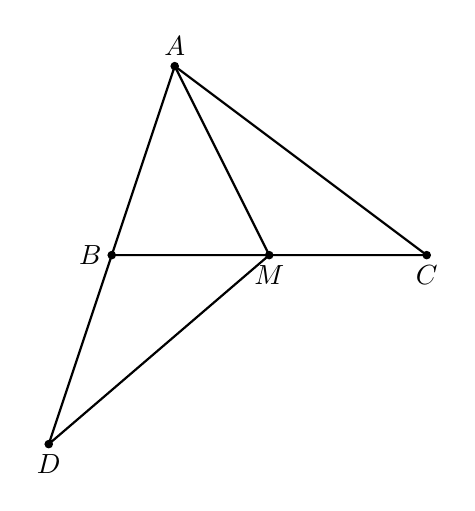
\begin{tikzpicture}[x=1cm,y=1cm,scale=0.8,thick]
		\coordinate (A) at (-1,2) ; 
		\coordinate (B) at (-2,-1) ; 
		\coordinate(D) at (-3, -4);
		\coordinate (C) at (3,-1) ; 
		\coordinate (M) at (0.5,-1) ;
		\draw (A)--(B)--(C)--(A);
		\draw (B)--(D)--(M)--(A) ; 
		\draw[fill] (A) circle (1.4pt) node[above] {$A$};
		\draw[fill] (B) circle (1.4pt) node[left] {$B$};
		\foreach \i in {C,D,M} \draw[fill] (\i) circle (1.4pt) node[below] {$\i$};
	\end{tikzpicture}
	\end{center}
	\begin{itemize}
		\item Giả thiết suy ra $B$ là trung điểm $AD$ và $M$ là trung điểm $BC$. 
		Nên ta có: $\vec{DM}=\vec{AM}-\vec{AD}=\dfrac{1}{2}(\vec{AB}+\vec{AC})-2\vec{AB}=-\dfrac{3}{2}\vec{AB}+\dfrac{1}{2}\vec{AC}$\\
	\end{itemize}
}
\end{bt}

% nguồn: TuLuan_Lop10_Dot2 (nhập 14/11/2026)
\begin{bt}%[0H5V3-4]%[Dự án đề kiểm tra HK1 NH22-23]%[Tạ Quang Bửu]%Lê Hùng Thắng%[ma:7f016900]
	Cho tam giác $A B C$ có trung tuyến $A M$. Gọi $I$ là trung điểm của $A M$ và $K$ là điểm trên cạnh $A C$ sao cho $A K=\dfrac{1}{3} A C$.
	\begin{enumerate}
	\item Chứng minh $\vec{B I}=\dfrac{1}{2} \vec{B A}+\dfrac{1}{4} \vec{B C}$.
	\item Tính $\vec{B K}$ theo $\vec{B A}, \vec{B C}$.
	\item Chứng minh ba điểm $B,~ I,~ K$ thẳng hàng.
	\end{enumerate}
	\dapso{a) $\vec{B I}=\dfrac{1}{2} \vec{B A}+\dfrac{1}{4} \vec{B C}$ ; b) $\vec{B K}=\dfrac{2}{3}\vec{BA}+\dfrac{1}{3}\vec{B C}$ ; c) Ba điểm $B,~ I,~ K$ thẳng hàng. }
	\loigiai{
	\begin{enumerate}
\immini{
	\item Vì $I$ là trung điểm của $AM$ nên ta có\\
	\allowdisplaybreaks
	$\begin{aligned}[t]
	 2\vec {BI} & = \vec{BA} +\vec{BM} \\
	\Rightarrow \vec{BI} & = \dfrac{1}{2}\vec{BA} +\dfrac{1}{2} \vec{BM}\\ 
	& = \dfrac{1}{2} \vec{BA}+\dfrac{1}{4} \vec{BC}.
	\end{aligned}$

}	
{\begin{tikzpicture}[scale=0.71,>=stealth, font=\footnotesize, line join=round, line cap=round]
	\path (0,4) coordinate (A)
	(-2,0) coordinate (B)
	(4,0) coordinate (C)
	($(B)!0.5!(C)$) coordinate (M)
	($(A)!0.5!(M)$) coordinate (I)
	($(A)!1/3!(C)$) coordinate (K);
	\draw (A)--(B)--(C)--(A)--(M) (B)--(K);
\foreach \d/\g in {A/150,B/180,C/0,M/-90,I/180,K/30} \fill (\d) circle (1pt) ++(\g: 3mm) node {$\d$};
\end{tikzpicture}
}
	\item Ta có \allowdisplaybreaks
	$\begin{aligned}[t]
	\vec {BK} & = \vec{BA} +\vec{AK} \\
	 & = \vec{BA} +\dfrac{1}{3} \vec{AC}\\ 
	& = \vec{BA}+\dfrac{1}{3}(\vec{BC}- \vec{BA})\\
	& = \dfrac{2}{3}\vec{BA}+\dfrac{1}{3} \vec{BC}.
	\end{aligned}$
	\item Ta có 
	$\vec {BI} =\dfrac{1}{2}\vec{BA}+\dfrac{1}{4} \vec{BC}$ và	$\vec {BK} =\dfrac{2}{3}\vec{BA}+\dfrac{1}{3} \vec{BC}$.\\
	Suy ra $\vec{B I} =\dfrac{3}{4} \vec{B K}$.\\
	Vậy ba điểm $B,~ I,~ K$ thẳng hàng.
\end{enumerate}
	}
\end{bt}

% nguồn: TuLuan_Lop10_Dot2 (nhập 14/11/2026)
\begin{bt}%[0H5V3-4]%[Dự án đề kiểm tra HKII NH22-23-Nguyễn Tài Tuệ]%[THPT Chuyên Lê QUý Đôn- Quảng Trị]%[ma:b4271522]
	 Cho tam giác $ABC$. Gọi $M$, $N$ là trung điểm $AB$, $BC$ và $P$ là điểm thỏa mãn $\overrightarrow{AP}=2 \overrightarrow{PC}$.
	 \begin{enumerate}
	 	\item  Chứng minh rằng $\overrightarrow{M P}=-\dfrac{1}{2}\overrightarrow{A B}+\dfrac{2}{3}\overrightarrow{A C}$.
	 	\item Biết $AB=3a$; $AC=6 a$, $A=60^{\circ}$. Tính $\left |\overrightarrow{M N}+\overrightarrow{MP}\right |$.
	 \end{enumerate}
 \loigiai{
 	\begin{center}
 		 \begin{tikzpicture}
 		 	\path
 		 	(0,0) coordinate (A)
 		 	(4,0) coordinate (C)
 		 	(1.5,2) coordinate (B)
 		 	($ (A)!0.5!(B) $) coordinate (M)
 		 	($ (B)!0.5!(C) $) coordinate (N)
 		 	($ (A)!2/3!(C) $) coordinate (P)
 		 	($ (A)!7/6!(C) $) coordinate (F)
 		 	($ (A)!-1/2!(B) $) coordinate (E)
 		 	($ (E)+(F)-(A) $) coordinate (K)
 		 	;
 		 	\draw(A)--(B)--(C)--cycle (A)--(E)--(K)--(F)--(C) (A)--(K) (M)--(P) ;
 		 	\foreach \p/\g in {A/180,B/90,C/80,M/180, N/0,P/-90,F/90,E/180,K/-90} \draw[fill] (\p) circle(.5pt)node [shift={(\g:.35)}] {$\p$};
 		 \end{tikzpicture}
 	\end{center}
 	
 \begin{enumerate}
 	\item Ta có $\overrightarrow{MP}=\overrightarrow{AP}-\overrightarrow{AM}=-\dfrac{1}{2}\overrightarrow{AB}+\dfrac{2}{3}\overrightarrow{AC}$.
 	\item Theo giả thiết, ta có\\ $\left |\overrightarrow{MN}+\overrightarrow{MP}\right |=\left|\dfrac{1}{2}\overrightarrow{AC}+\left(-\dfrac{1}{2}\overrightarrow{AB}+\dfrac{2}{3}\overrightarrow{AC}\right)\right|=\left|-\dfrac{1}{2}\overrightarrow{AB}+\dfrac{7}{6}\overrightarrow{AC}\right|$.\\
 	Dựng điểm $ E $ đối xứng với $ M $ qua $ A $ và dựng điểm $ F $ sao cho $\overrightarrow{AF}=\dfrac{7}{6}\overrightarrow{AC}$ và điểm $ K $ sao cho $ AEKF $ là hình bình hành.\\
 	Ta có
 	$ \left|-\dfrac{1}{2}\overrightarrow{AB}+\dfrac{7}{6}\overrightarrow{AC}\right|   =\left |\overrightarrow{AE}+\overrightarrow{AF}\right |=\left |\overrightarrow{AK}\right |=AK$.\\
 	Ta có $ AE=\dfrac{1}{2}AB =\dfrac{3a}{2}$ và $ EK=AF=\dfrac{7}{6}AC =7a$,  $ \widehat{AEK} =60^\circ$.\\
 	Áp dụng đinh lí cô-sin vào tam giác $ AEK $ có\\
 	$ AK^2=AE^2+EK^2-2AE\cdot EK\cdot \cos \widehat{AEK} =\left(\dfrac{3a}{2}\right)^2+\left(7a\right)^2-2\cdot \dfrac{3a}{2}\cdot7a\cdot\dfrac{1}{2}=\dfrac{163a^2}{4}$\\
 	$ \Rightarrow AK=\dfrac{a\sqrt{163}}{2}  $.\\
 	Vậy $\left |\overrightarrow{MN}+\overrightarrow{MP}\right |=\dfrac{a\sqrt{163}}{2}$.
 	
 \end{enumerate}
 }
\end{bt}

% nguồn: TuLuan_Lop10_Dot2 (nhập 14/11/2026)
\begin{bt}%[0H5V3-4]%[Dự án đề kiểm tra HKII NH22-23- Nguyễn Ngọc Nguyên]%[THPT Quế Sơn - Quảng Nam]%[ma:f8771bb0]
	Cho tam giác $ABC$ có trung tuyến $AI$. Gọi $M$ là trung điểm của $AI$, $H$ là điểm thuộc cạnh $AC$ sao cho $AH=4HC$. Chứng minh rằng $20\overrightarrow{MH}=11\overrightarrow{AC}-5\overrightarrow{AB}$.
	\loigiai{
\immini{
Ta có
\begin{eqnarray*}
	\overrightarrow{MH}&=&\overrightarrow{AH}-\overrightarrow{AM} = \dfrac{4}{5}\overrightarrow{AC}-\dfrac{1}{2}\overrightarrow{AI} \\
	 &=& \dfrac{4}{5} \overrightarrow{AC} - \dfrac{1}{2} \cdot \dfrac{1}{2} \left(\overrightarrow{AB}+\overrightarrow{AC}\right)=\dfrac{11}{20}\overrightarrow{AC}-\dfrac{1}{4}\overrightarrow{AB}
\end{eqnarray*}
Từ đó suy ra $20\overrightarrow{MH}=11\overrightarrow{AC}-5\overrightarrow{AB}$.
}
{
\begin{tikzpicture}[scale=0.85,>=stealth, font=\footnotesize, line join=round, line cap=round]
	\path 
	(0,0) coordinate (A)
	(-3,-5) coordinate (B)
	(4,-3) coordinate (C)
	($(C)!0.5!(B)$) coordinate (I)
	($(A)!0.5!(I)$) coordinate (M)
	($(A)!0.8!(C)$) coordinate (H)
	;
	\draw (A)--(B)--(C)--cycle;
	\draw (A)--(I) (M)--(H);
	\foreach \t/\g in {A/90,B/-90,C/-90,I/-90,M/180,H/45}{\draw[fill=white] (\t) circle (1pt) node[shift={(\g:8pt)},font=\footnotesize]{$ \t $};
	}
	\foreach \x/\y in {B/I,C/I}{
		\path (\x)--(\y) node[midway,sloped]{\tikz{\draw[thick,teal] (-90:2pt)--(90:2pt);}};
	}
	\foreach \x/\y in {A/M,M/I}{
	\path (\x)--(\y) node[midway,sloped]{\tikz{\draw[shift={(-0.65pt,0)}](-90:2pt)--(90:2pt) [shift={(0.65pt,0)}](-90:2pt)--(90:2pt);}};
}
\end{tikzpicture}
}		
	}
\end{bt}

% nguồn: TuLuan_Lop10_Dot2 (nhập 14/11/2026)
\begin{bt}%[0H5V3-4]%[Dự án đề kiểm tra HKI NH22-23- Nguyễn Văn Sang]%[THPT Trần Khai Nguyên]%[ma:18be79bf]
	Cho tam giác $ABC$, lấy các điểm $M$, $N$, $P$ sao cho $\overrightarrow{M A}+2 \overrightarrow{M B}=\overrightarrow{0}$; $4 \overrightarrow{N B}+\overrightarrow{N C}=\overrightarrow{0}$; $2 \overrightarrow{P A}-\overrightarrow{P C}=\overrightarrow{0}$.
	\begin{enumerate}
		\item Biểu thị mỗi vectơ $\overrightarrow{P M}$, $\overrightarrow{P N}$ theo hai vectơ $\overrightarrow{A B}$, $\overrightarrow{A C}$.
		\item Chứng minh ba điểm $M$, $N$, $P$ thẳng hàng.
	\end{enumerate}
	\dapso{ a) $\overrightarrow{PM}=\dfrac{2}{3} \overrightarrow{AB}+\overrightarrow{AC}$; $\overrightarrow{PN}=\dfrac{4}{5} \overrightarrow{AB}+ \dfrac{6}{5} \overrightarrow{AC}$.}
	\loigiai{
	\begin{enumerate}
		\item Biểu thị mỗi vectơ $\overrightarrow{P M}$, $\overrightarrow{P N}$ theo hai vectơ $\overrightarrow{A B}$, $\overrightarrow{A C}$.\\
		Ta có 
		\begin{itemize}
			\item 	$\overrightarrow{M A}+2 \overrightarrow{M B}=\overrightarrow{0}$ nên $M$ thuộc đoạn $AB$ và $AM=2MB$.
			\item $4 \overrightarrow{N B}+\overrightarrow{N C}=\overrightarrow{0}$ nên $N$ thuộc đoạn $BC$ và $NC=4BN$.
			\item $2 \overrightarrow{P A}-\overrightarrow{P C}=\overrightarrow{0}$ nên $A$ là trung điểm $PC$.
		\end{itemize}
	\immini
	{
	Ta có 
	\begin{eqnarray*}
		\overrightarrow{PM}&=&\overrightarrow{PA}+\overrightarrow{AM}\\
						   &=&\overrightarrow{AC}+\dfrac{2}{3}\overrightarrow{AB}.\qquad(1)
	\end{eqnarray*}
	Ta có
	\begin{eqnarray*}
		\overrightarrow{PN}&=&\overrightarrow{PA}+\overrightarrow{AN}=\overrightarrow{AC}+\overrightarrow{AB}+\overrightarrow{BN}\\
		&=&\overrightarrow{AC}+\overrightarrow{AB}+\dfrac{1}{5}\left( \overrightarrow{BC}\right)\\
		&=&\overrightarrow{AC}+\overrightarrow{AB}+\dfrac{1}{5}\left(\overrightarrow{AC}-\overrightarrow{AB}\right)\\
		&=&\dfrac{4}{5} \overrightarrow{AB}+ \dfrac{6}{5} \overrightarrow{AC}.\qquad(2)
	\end{eqnarray*}
	}
	{
	\begin{tikzpicture}[>=stealth,line join=round,line cap=round,font=\footnotesize,scale=.6]
		%\draw[thin,gray!50,step=1cm] (-5,-5) grid (5,5);
		\fill (0,3)coordinate(A) circle (1pt) node[above]{$A$};
		\fill (-2,0)coordinate(B) circle (1pt) node[below]{$B$};
		\fill (3,0)coordinate(C) circle (1pt) node[below]{$C$};
		\coordinate (M) at ($(A)!2/3!(B)$); 
		\coordinate (N) at ($(C)!4/5!(B)$); 
		\coordinate (P) at ($(C)!2/1!(A)$); 
		\fill (M) node[left]{$M$};
		\fill (N) node[below]{$N$};
		\fill (P) circle (1pt) node[left]{$P$};
		\foreach \i in {1,...,4} {
			\coordinate (N\i) at ($(C)!\i/5!(B)$);
			\node[fill,circle,inner sep=.7pt] at (N\i) {};
		}
		\foreach \i in {1,...,2} {
			\coordinate (M\i) at ($(A)!\i/3!(B)$);
			\node[fill,circle,inner sep=.7pt] at (M\i) {};
		}
		\draw(A)--(B)--(C)--(P) ;
	\end{tikzpicture}
	}\noindent
	\item Chứng minh ba điểm $M$, $N$, $P$ thẳng hàng.\\
	Từ $(1)\Leftrightarrow 3\overrightarrow{PM}=2\overrightarrow{AB}+3\overrightarrow{AC}$.\\
	Từ $(2)\Leftrightarrow \dfrac{5}{2}\overrightarrow{PN}=2\overrightarrow{AB}+3\overrightarrow{AC}$.\\
	Suy ra $3\overrightarrow{PM}=\dfrac{5}{2}\overrightarrow{PN} \Leftrightarrow\overrightarrow{PM}=\dfrac{5}{6}\overrightarrow{PN}$ hay $P$, $M$, $N$ thẳng hàng.
\end{enumerate}
	}
\end{bt}

% nguồn: TuLuan_Lop10_Dot2 (nhập 14/11/2026)
\begin{bt}%[0H5V3-4]%[Dự án đề kiểm tra HKII NH22-23- Nguyễn Cường%[Sở GD-ĐT Hà Nam]%[ma:d0843acb]
Cho tam giác $ABC$ có trọng tâm $G$. Gọi $I$ là trung điểm $AG$ và $M$, $N$ lần lượt là các điểm thỏa mãn $\overrightarrow{MN}=4\overrightarrow{MA}+\overrightarrow{MB}+\overrightarrow{MC}$. Chứng minh rằng ba điểm $M$, $I$, $N$ thẳng hàng.
\loigiai{
\immini
{
Ta có 
\allowdisplaybreaks
\begin{eqnarray*}
	\overrightarrow{MN}&=&4\overrightarrow{MA}+\overrightarrow{MB}+\overrightarrow{MC}\\
	&=&4\left(\overrightarrow{MI}+\overrightarrow{IA}\right)+\overrightarrow{MI}+\overrightarrow{IB}+\overrightarrow{MI}+\overrightarrow{IC}\\
	&=&6\overrightarrow{MI}+4\overrightarrow{IA}+\overrightarrow{IB}+\overrightarrow{IC}
\end{eqnarray*}
Gọi $D$ là trung điểm $BC$, ta có $\overrightarrow{IB}+\overrightarrow{IC}=2\overrightarrow{ID}$.\\
Mà $I$ là trung điểm $AG$ nên $\overrightarrow{ID}=2\overrightarrow{AI}$.\\
Do đó, $4\overrightarrow{IA}+\overrightarrow{IB}+\overrightarrow{IC}=4\overrightarrow{IA}+4\overrightarrow{AI}=\overrightarrow{0}$.\\
Suy ra $\overrightarrow{MN}=6\overrightarrow{MI}$, hay ba điểm $M$, $I$, $N$ thẳng hàng.
}
{
\begin{tikzpicture}[font=\footnotesize, line join=round, line cap=round, >=stealth,scale=1]
	\path (0:0) coordinate (B)
	+(0:5) coordinate (C)
	+(70:3) coordinate (A)
	($(B)!.5!(C)$)coordinate (D)
	($(A)!2/3!(D)$)coordinate (G)
	($(A)!.5!(G)$)coordinate (I)
	;
	\draw (A)--(B)--(C)--cycle
	;
	\draw[->](I)--(B);
	\draw[->](I)--(A);
	\draw[->](I)--(C);
	\draw[->](I)--(D);
	\foreach \x/\g in {B/180,C/0,A/90,D/-90,G/45,I/45}
	\fill (\x) circle (1pt)
	+(\g:3mm) node{$\x$};
\end{tikzpicture}

}
}
\end{bt}

% nguồn: TuLuan_Lop10_Dot2 (nhập 14/11/2026)
\begin{bt}%[0H5C3-4]%[Dự án đề kiểm tra HKI NH22-23- NGUYỄN VĂN SƠN %[SGD HÀ NAM]%[ma:b8fdf991]
Cho tam giác đều $ABC$. Gọi $M$, $N$, $P$ lần lượt là các điểm thoả mãn\\ $\overrightarrow{BM}=k\overrightarrow{BC}$, $3\overrightarrow{AN}=2\overrightarrow{AB}$, $5\overrightarrow{AP}=2\overrightarrow{AC}.$\\
	\begin{enumerate}
		\item Biểu diễn $\overrightarrow{AM}$ theo hai véc-tơ $\overrightarrow{AB}$, $\overrightarrow{AC}$.\\
		\item Tìm $k$ để hai đường thẳng $AM$, $NP$ vuông góc với nhau.
	\end{enumerate}
\loigiai{
	
	\begin{enumerate}
	\item  Từ giả thiết $\overrightarrow{BM}=k\overrightarrow{BC}$ 
	$\Rightarrow \overrightarrow{AM}-\overrightarrow{AB}=k(\overrightarrow{AC}-\overrightarrow{AB})$ $\Rightarrow  \overrightarrow{AM}=(1-k) \overrightarrow{AB}+k\overrightarrow{AC}$.
	\item Theo giả thiết $3\overrightarrow{AN}=2\overrightarrow{AB} \Rightarrow$ $3(\overrightarrow{AP}+\overrightarrow{PN})=2\overrightarrow{AB}$$\Rightarrow$ $ 3\overrightarrow{PN}=2\overrightarrow{AB}-3\overrightarrow{AP} \quad $ (1).\\
	Mặt khác $5\overrightarrow{AP}=2\overrightarrow{AC}$$\Rightarrow$$\overrightarrow{AP}=\dfrac{2}{5}\overrightarrow{AC}\quad $ (2).\\
	Từ (1) và (2) ta có: $ \overrightarrow{PN}=\dfrac{2}{3}\overrightarrow{AB}-\dfrac{2}{5}\overrightarrow{AC}$.\\
	Để $AM$ và $NP$ vuông góc với nhau thì $ \overrightarrow{AM}.\overrightarrow{PN}=0$\\
	$\Leftrightarrow \left((1-k)\overrightarrow{AB}+k\overrightarrow{AC}\right)\left( \dfrac{2}{3}\overrightarrow{AB}-\dfrac{6}{5}\overrightarrow{AC}\right)=0$\quad (*).\\
	Đặt $AB=AC=BC=a$. Khi đó ta có $\overrightarrow{AB}.\overrightarrow{AC} = \left| \overrightarrow{AB}\right|.\left| \overrightarrow{AC}\right|.\cos 60^\circ = \dfrac{a^2}{2}$. \\
	Từ (*) ta có $\dfrac{2(1-k)}{3}\cdot a^2-\dfrac{6(1-k)}{5}\cdot a^2.\dfrac{1}{2}+\dfrac{2k}{3}.a^2\cdot\dfrac{1}{2}-\dfrac{6k}{5}\cdot a^2=0$
	$\Rightarrow k=\dfrac{7}{8}$.	
	\end{enumerate}
}
\end{bt}

% nguồn: TuLuan_Lop10_Dot2 (nhập 14/11/2026)
\begin{bt}%[0H5H3-4]%[Dự án đề kiểm tra HKI NH22-23- Thành Đức Trung]%[THPT Nguyễn Du - Hồ Chí Minh]%[ma:392e4aa3]
Cho tam giác $ABC$, các điểm $M$, $N$ thỏa mãn $\overrightarrow{MB}=\dfrac{1}{2}\overrightarrow{BC}$, $\overrightarrow{AN}=3\overrightarrow{NB}$. Hãy biểu thị $\overrightarrow{MN}$ theo hai véc-tơ $\overrightarrow{AB}$ và $\overrightarrow{BC}$.
\loigiai
{Do $\overrightarrow{AN}=3\overrightarrow{NB}$ nên $\overrightarrow{BN}=-\dfrac{1}{4}\overrightarrow{AB}$.\\
Ta có 
\[\overrightarrow{MN}=\overrightarrow{MB}+\overrightarrow{BN}=\dfrac{1}{2}\overrightarrow{BC}-\dfrac{1}{4}\overrightarrow{AB}.\]
Vậy $\overrightarrow{MN}=\dfrac{1}{2}\overrightarrow{BC}-\dfrac{1}{4}\overrightarrow{AB}$.
}
\end{bt}

% nguồn: TuLuan_Lop10_Dot2 (nhập 14/11/2026)
\begin{bt}%[0H5H3-4]%[Dự án đề kiểm tra HK1 22-23-Nhật Thiện]%[Trường THPT PHÙNG KHẮC KHOAN, HÀ NỘI]%[ma:882d707a]
	Cho tam giác $ABC$. Gọi $I$, $J$ là hai điểm xác định bởi các đẳng thức $\vec{IA}=2\vec{IB}$, $3\vec{JA}+2\vec{JC}=\vec{0}$. Hãy phân tích $\vec{IJ}$ theo $\vec{AB}$ và $\vec{AC}$.
	\loigiai{
	Ta có $\vec{IJ}=\vec{IA}+\vec{AJ}$.\\
	Mặt khác $\vec{IA}=-2\vec{AB}$ và $\vec{AJ}=\dfrac{2}{5}\vec{AC}$.\\
	Suy ra $\vec{IJ}=\dfrac{2}{5}\vec{AC}-2\vec{AB}$.\\
	Vậy $\vec{IJ}=\dfrac{2}{5}\vec{AC}-2\vec{AB}$.
}
\end{bt}

% nguồn: TuLuan_Lop10_Dot2 (nhập 14/11/2026)
\begin{bt}%[0H5V3-4] % KIEM_TRA%[Dự án đề kiểm tra HKII NH22-23-BC Tuan]%[THPT Lương Thế Vinh Quảng Nam]%[ma:d3ea4a9a]
	Cho tam giác đều $ABC$ cạnh $a$, trên các cạnh $BC$, $CA$, $AB$ lấy các điểm $M$, $N$, $P$ sao cho
	$\overrightarrow{BM}=\dfrac{1}{3} \overrightarrow{BC}$, $\overrightarrow{AN}=-\dfrac{1}{2} \overrightarrow{CN}$, $\overrightarrow{AP}=m \overrightarrow{AB}$ $(0<m<a)$. Hãy phân tích véc-tơ $\overrightarrow{AM}$ theo $\overrightarrow{AB}$, $\overrightarrow{AC}$ và tìm $m$ biết $A M$ vuông góc với $P N$.
	\loigiai{
		Ta có $\overrightarrow{A M}=\overrightarrow{AB}+\overrightarrow{BM}=\overrightarrow{AB}+\dfrac{1}{3} \overrightarrow{BC}=\overrightarrow{AB}+\dfrac{1}{3}\left(\overrightarrow{AC}-\overrightarrow{AB}\right)=\dfrac{2}{3}\overrightarrow{AB}+\dfrac{1}{3}\overrightarrow{AC}$.\\
		$A M$ vuông góc với $P N$ khi và chỉ khi
		$$\begin{aligned} & \overrightarrow{A M} \cdot \overrightarrow{P N}=0 \\ & \Leftrightarrow\left(\dfrac{2}{3} \overrightarrow{AB}+\dfrac{1}{3} \overrightarrow{AC}\right) \cdot \left(\overrightarrow{P A}+\overrightarrow{A N}\right)=0 \\ & \Leftrightarrow\left(\dfrac{2}{3} \overrightarrow{AB}+\dfrac{1}{3} \overrightarrow{AC}\right)\left(-m \overrightarrow{AB}+\dfrac{1}{3} \overrightarrow{AC}\right)=0 \\ & \Leftrightarrow-\dfrac{2}{3} m \overrightarrow{AB}^2+\dfrac{1}{9} \overrightarrow{AC}^2-\dfrac{1}{3} m \overrightarrow{AB} \cdot \overrightarrow{AC}+\dfrac{2}{9} \overrightarrow{AB} \cdot \overrightarrow{AC}=0 \\ & \Leftrightarrow-\dfrac{2}{3} m \cdot a^2+\dfrac{1}{9} a^2-\dfrac{1}{3} m \cdot a^2 \cdot \cos 60^\circ+\dfrac{2}{9} \cdot a^2 \cdot \cos 60^\circ=0 \\ & \Leftrightarrow m=\dfrac{4}{15}.\end{aligned}$$
		Vậy $m=\dfrac{4}{15}$.
	}
\end{bt}

% nguồn: TuLuan_Lop10_Dot2 (nhập 14/11/2026)
\begin{bt}%[0H5H3-4] % KIEM_TRA%[Tex hóa SBT CT,T7/22, Phạm Doãn Lê Bình]%[ma:d095e3ad]
	Cho ba điểm $O$, $M$, $N$ và số thực $k$. Lấy các điểm $M'$ và $N'$ sao cho $\overrightarrow{OM'}=k\overrightarrow{OM}$; $\overrightarrow{ON'}=k\overrightarrow{ON}$. Chứng minh rằng $\overrightarrow{M'N'}=k\overrightarrow{MN}$.
	\loigiai{
		Ta có 
		\begin{eqnarray*}
			&\overrightarrow{M'N'}& = \overrightarrow{ON'}-\overrightarrow{OM'}\\
			& & = k\overrightarrow{ON}-k\overrightarrow{OM}\\
			& & = k\left( \overrightarrow{ON}-\overrightarrow{OM}\right) = k\overrightarrow{MN}.
		\end{eqnarray*}
	}
\end{bt}

% nguồn: TuLuan_Lop10_Dot2 (nhập 14/11/2026)
\begin{bt}%[0H5H3-4]%[Tex hóa SBT CT,T7/22, Phạm Doãn Lê Bình]%[ma:1d12a809]
	Cho tam giác $ABC$, $O$ là điểm sao cho ba véc-tơ $\overrightarrow{OA}$, $\overrightarrow{OB}$, $\overrightarrow{OC}$ có độ dài bằng nhau và $\overrightarrow{OA}+\overrightarrow{OB}+\overrightarrow{OC}=\overrightarrow{0}$. Tính các góc $\widehat{AOB}$, $\widehat{BOC}$, $\widehat{COA}$.
	\loigiai{
		Ta có $OA=OB=OC$, suy ra $O$ là tâm đường tròn ngoại tiếp tam giác $ABC$.\\
		Ta lại có $\overrightarrow{OA}+\overrightarrow{OB}+\overrightarrow{OC}=\overrightarrow{0}$, suy ra $O$ cũng là trọng tâm tam giác $ABC$.\\
		Vậy $ABC$ là tam giác đều, suy ra $\widehat{AOB}=\widehat{BOC}=\widehat{COA}=120^\circ$.
	}
\end{bt}

% nguồn: TuLuan_Lop10_Dot2 (nhập 14/11/2026)
\begin{bt}%[0H5V3-4]%[Đề kiểm tra HK1 môn Toán 11 trường THPT Phùng Khắc Khoan]%[Nguyễn Quang Hiệp, 10EX-HK1-2223]%[ma:a14f1674]
	Cho tam giác $A B C$. Gọi $I, J$ là hai điểm xác định bởi các đẳng thức $\overrightarrow{I A}=2 \overrightarrow{I B}$,\break $3 \overrightarrow{J A}+2 \overrightarrow{J C}=\overrightarrow{0}$. Hãy phân tích $\overrightarrow{I J}$ theo $\overrightarrow{A B}$ và $\overrightarrow{A C}$.
	\loigiai{
		\immini{
			Ta có $\overrightarrow{I J}=\overrightarrow{I A}+\overrightarrow{A J}$ và $\overrightarrow{I A}=-2 \overrightarrow{A B}$.\\
			Lại có $\overrightarrow{A J}=\dfrac{2}{5} \overrightarrow{A C}$.\\
			Suy ra $\overrightarrow{I J}=\dfrac{2}{5} \overrightarrow{A C}-2 \overrightarrow{A B}$.\\
			Vậy $\overrightarrow{I J}=\dfrac{2}{5} \overrightarrow{A C}-2 \overrightarrow{A B}$.    
		}{
			\begin{tikzpicture}[>=stealth,line join=round,line cap=round,font=\footnotesize,scale=1.5]
				\tikzset{
					% Khai báo độ dài ba cạnh tam giác
					declare function={a=4;b=3;c=1.5;}
				}
				% Định lí hàm số cos
				\pgfmathsetmacro{\goc}{
					acos((a*a+c*c-b*b)/(2*a*c))
				}
				% Vẽ tam giác 
				\draw (0,0)coordinate (A)--+(0:a)coordinate (C)--+(-\goc:c)coordinate (B)--cycle
				(B)--($(A)!2!(B)$)coordinate (I)--($(A)!2/5!(C)$)coordinate (J) 
				;
				\foreach \point/\goc in {A/180,B/-110,C/-10,J/90,I/-60}{
					\draw[fill=black](\point)circle(0.8pt)+(\goc:2mm)node[scale=.8]{$\point$};
				}
			\end{tikzpicture}   
		}
		
	}
\end{bt}

% nguồn: TuLuan_Lop10_Dot2 (nhập 14/11/2026)
\begin{bt}%[0H5V3-4]%[ma:c14eebb8]
	Cho tam giác $ABC$, trên cạnh $BC$ lấy $M$ sao cho $BM=3CM$, trên đoạn $AM$ lấy $N$ sao cho $2AN=5MN$. Gọi $G$ là trọng tâm tam giác $ABC$.
	\begin{enumerate}
		\item Phân tích các véc-tơ $\overrightarrow{AM},\, \overrightarrow{BN}$ qua các véc-tơ $\overrightarrow{AB}$ và $\overrightarrow{AC}$.
		\item Phân tích các véc-tơ $\overrightarrow{GC},\,\overrightarrow{MN}$ qua các véc-tơ $\overrightarrow{GA}$ và $\overrightarrow{GB}$.
	\end{enumerate}
	\loigiai{
		\begin{center}
			\begin{tikzpicture}
				\coordinate[label=left:$B$] (B) at (0,0);
				\coordinate[label=below:$C$] (C) at (4,0);
				\coordinate[label=above:$A$] (A) at (1,3);
				\coordinate[label=below:$M$] (M) at ($(B)!.75!(C)$ );
				\coordinate[label=left:$N$] (N) at ($(A)!5/7!(M)$ );
				\coordinate (I) at ($(B)!0.25!(C)$ );
				\coordinate (G) at ($(B)!0.5!(C)$ );
				\draw (A)--(M);
				\draw (A)--(B)--(C)--cycle;
				\fill (A)circle(1.5pt) (B)circle(1.5pt) (C)circle(1.5pt) (I)circle(1.5pt) (M)circle(1.5pt) (G)circle(1.5pt) (N)circle(1.5pt);
			\end{tikzpicture}   
		\end{center}
		\begin{enumerate}
			\item Theo giả thiết ta có $\overrightarrow{BM}=\dfrac{3}{4}\overrightarrow{BC}$ và $\overrightarrow{AN}=\dfrac{5}{7}\overrightarrow{AM}$.\\
			suy ra 
			\begin{eqnarray*}
				\overrightarrow{AM}&=&\overrightarrow{AB}+\overrightarrow{BM}=\overrightarrow{AB}+\dfrac{3}{4}\overrightarrow{BC}\\
				&=&\overrightarrow{AB}+\dfrac{3}{4}\left(\overrightarrow{AC}-\overrightarrow{AB}\right)=\dfrac{1}{4}\overrightarrow{AB}+\dfrac{3}{4}\overrightarrow{AC}.\\
				\overrightarrow{BN}&=&\overrightarrow{BA}+\overrightarrow{AN}=-\overrightarrow{AB}+\dfrac{5}{7}\overrightarrow{AM}\\
				&=&-\overrightarrow{AB}+\dfrac{5}{7}\left(\dfrac{1}{4}\overrightarrow{AB}+\dfrac{3}{4}\overrightarrow{AC}\right)=-\dfrac{23}{28}\overrightarrow{AB}+\dfrac{15}{28}\overrightarrow{AC}.    
			\end{eqnarray*}
			\item Vì $G$ là trọng tâm tam giác $ABC$ nên $\overrightarrow{GA}+\overrightarrow{GB}+\overrightarrow{GC}=\overrightarrow 0 $ suy ra $\overrightarrow{GC}=-\overrightarrow{GA}-\overrightarrow{GB}$.\\
			Ta có 
			\begin{eqnarray*}
				\overrightarrow{MN}&=&-\dfrac{2}{7}\overrightarrow{AM}=-\dfrac{2}{7}\left(\dfrac{1}{4}\overrightarrow{AB}+\dfrac{3}{4}\overrightarrow{AC}\right)\\
				&=&-\dfrac{1}{14}\left(\overrightarrow{GB}-\overrightarrow{GA}\right)-\dfrac{3}{14}\left(\overrightarrow{GC}-\overrightarrow{GA}\right)\\
				&=&-\dfrac{1}{14}\left(\overrightarrow{GB}-\overrightarrow{GA}\right)-\dfrac{3}{14}\left(-\overrightarrow{GA}-\overrightarrow{GB}-\overrightarrow{GA}\right)\\
				&=&\dfrac{1}{2}\overrightarrow{GA}+\dfrac{1}{7}\overrightarrow{GB}.
			\end{eqnarray*}
		\end{enumerate}     
	}  
\end{bt}

% nguồn: TuLuan_Lop10_Dot2 (nhập 14/11/2026)
\begin{bt}%[0H5V3-4]%[ma:84d06bcb]
	Cho hình bình hành $ABCD$. Gọi $M, \,N$ lần lượt là hai điểm nằm trên hai cạnh $AB$ và $CD$ sao cho $AB=3AM,\,CD=2CN$ và $G$ là trọng tâm tam giác $MNB$. Phân tích các véc-tơ $\overrightarrow{AN},\,\overrightarrow{MN},\,\overrightarrow{AG}$ qua các véc-tơ $\overrightarrow{AB}$ và $\overrightarrow{AC}$.
	\loigiai{
		\begin{center}
			\begin{tikzpicture}[>=stealth,x=1cm,y=1cm,scale=0.65]
				\coordinate[label=below :$D$](D) at (0,0);
				\coordinate[label=below :$A$](A) at (5,0);
				\coordinate[label=above:$C$](C) at (2,4);
				\coordinate[label=above:$B$](B) at (7,4);
				\coordinate[label=right:$M$] (M) at ($(A)!1/3!(B)$); 
				\coordinate[label=left:$N$] (N) at ($(C)!1/2!(D)$); 
				\coordinate(I) at ($(M)!1/2!(B)$); 
				\coordinate[label=right :$G$] (G) at ($(N)!2/3!(I)$); 
				\foreach \toado in {(A),(B),(C),(N),(M),(D),(G)}{
					\fill \toado circle (1.5pt);}
				\draw (C)--(B)--(A)--(D)--(C) (M)--(N)--(B);
			\end{tikzpicture}
		\end{center}
		Ta có
		\begin{eqnarray*}
			\overrightarrow{AN}&=&\overrightarrow{AC}+\overrightarrow{CN}=\overrightarrow{AC}-\dfrac{1}{2}\overrightarrow{AB}\\
			\overrightarrow{MN}&=&\overrightarrow{MA}+\overrightarrow{AN}=-\dfrac{1}{3}\overrightarrow{AB}+\overrightarrow{AC}-\dfrac{1}{2}\overrightarrow{AB}\\
			&=&-\dfrac{5}{6}\overrightarrow{AB}+\overrightarrow{AC}. 
		\end{eqnarray*}
		Vì $G$ là trọng tâm tam giác $MNB$ nên
		$$3\overrightarrow{AG}=\overrightarrow{AM}+\overrightarrow{AN}+\overrightarrow{AB}=\dfrac{1}{3}\overrightarrow{AB}+\left(\overrightarrow{AC}-\dfrac{1}{2}\overrightarrow{AB}\right)+\overrightarrow{AB}=\dfrac{5}{6}\overrightarrow{AB}+\overrightarrow{AC}$$
		Suy ra $\overrightarrow{AG}=\dfrac{5}{18}\overrightarrow{AB}+\dfrac{1}{3}\overrightarrow{AC}$.
	}  
\end{bt}

% nguồn: TuLuan_Lop10_Dot2 (nhập 14/11/2026)
\begin{bt}%[0H5V3-4]%[ma:42896316]
	Cho tứ giác $ABCD$. Với số $k$ tùy ý, lấy các điểm $M$ và $N$ sao cho $\overrightarrow{AM}=k\overrightarrow{AB},\,\overrightarrow{DN}=k\overrightarrow{DC}$. Tìm tập hợp các trung điểm $I$ của đoạn thẳng $MN$ khi $k$ thay đổi.
	\loigiai{
		\begin{center}
			\begin{tikzpicture}
				\coordinate (A) at (0,0);
				\coordinate (B) at (5,0);
				\coordinate (C) at (3,3);
				\coordinate (D) at (1,2);
				\coordinate (M) at ($ (A)!0.3!(B) $);
				\coordinate (N) at ($ (D)!0.3!(C) $);
				\coordinate (O) at ($ (A)!0.5!(D) $);
				\coordinate (O') at ($ (C)!0.5!(B) $);
				\draw[fill] (A) circle(1pt) node[below]{$ A $} -- (B)circle(1pt) node[below]{$ B $}-- (C)circle(1pt) node[above]{$ C $}-- (D)circle(1pt) node[above]{$ D $} -- (A) (O)circle(1pt) node[left]{$ O $}--(O')circle(1pt) node[right]{$ O' $};
				\draw[fill] (M)node[below]{$ M $} circle(1pt) -- (N) node[above]{$ N $} circle(1pt);
			\end{tikzpicture}   
		\end{center}
		Gọi $O, \,O'$ lần lượt là trung điểm của $AD$ và $BC$, ta có\\
		$\overrightarrow{AB}=\overrightarrow{AO}+\overrightarrow{OO'}+\overrightarrow{O'B}$ và $\overrightarrow{DC}=\overrightarrow{DO}+\overrightarrow{OO'}+\overrightarrow{O'C}$\\
		Suy ra $\overrightarrow{AB}+\overrightarrow{DC}=2\overrightarrow{OO'}$.\\
		Tương tự vì $O, \,I$ lần lượt là trung điểm của $AD$ và $MN$ nên
		$$\overrightarrow{AM}+\overrightarrow{DN}=2\overrightarrow{OI}.$$
		Do đó $\overrightarrow{OI}=\dfrac{1}{2}\left(k\overrightarrow{AB}+k\overrightarrow{DC}\right)=k\overrightarrow{OO'}$.\\
		Vậy khi $k$ thay đổi, tập hợp điểm $I$ là đường thẳng $OO'$.  
	}
\end{bt}

% nguồn: TuLuan_Lop10_Dot2 (nhập 14/11/2026)
\begin{bt}%[0H5V3-4]%[ma:9c124e12]
	Chứng minh rằng ba điểm $A$, $B$, $C$ thẳng hàng khi và chỉ khi hai véc-tơ $\overrightarrow{AB}$, $\overrightarrow{AC}$ cùng phương.
	\loigiai{
		\begin{itemize}
			\item Giả sử ba điểm $A$, $B$, $C$ thẳng hàng. Khi đó, chúng cùng thuộc một đường thẳng $d$. Vậy hai véc-tơ $\overrightarrow{AB}$, $\overrightarrow{AC}$ có cùng giá là $d$. Suy ra chúng cùng phương.\\
			\item Giả sử hai véc-tơ $\overrightarrow{AB}$, $\overrightarrow{AC}$ cùng phương. Khi đó, chúng có cùng giá hoặc có hai giá song song với nhau. Mặt khác, giá của các véc-tơ trên đều đi qua $A$ nên chúng trùng nhau. Vậy $A$, $B$, $C$ thẳng hàng.
		\end{itemize}
	}
\end{bt}

% nguồn: TuLuan_Lop10_Dot2 (nhập 14/11/2026)
\begin{bt}%[0H5H3-4]%[ma:13eaaf05]
	Cho $\triangle ABC$ có $M$ là trung điểm của cạnh $BC$. Các điểm $D$, $E$ thỏa mãn đẳng thức $\overrightarrow{BD}= 4 \overrightarrow{BA}$, $\overrightarrow{AE}= 3 \overrightarrow{AC}$. Chứng minh $DE \parallel AM$.
	\loigiai{
		\immini
		{
			Ta có $M$ là trung điểm của $BC$ nên $\overrightarrow{AM}= \dfrac{1}{2}\left( \overrightarrow{AB}+ \overrightarrow{AC}\right)$.\\
			Vì $\overrightarrow{BD}= 4 \overrightarrow{BA} \Rightarrow \overrightarrow{AD}= -3\overrightarrow{AB}$. Do đó\\
			$\overrightarrow{DE}= \overrightarrow{AE}- \overrightarrow{AD}= 3 \overrightarrow{AC} + 3\overrightarrow{AB}= 6 \overrightarrow{AM}$.\\
			Suy ra hai véc-tơ $\overrightarrow{DE}$ và $\overrightarrow{AM}$ cùng phương. Vậy $DE \parallel AM$.
		}
		{
			\begin{tikzpicture}[scale=.7, font=\footnotesize, line join=round, line cap=round, >=stealth]
				\coordinate (A) at (0,0);
				\coordinate (B) at (-.5,-1);
				\coordinate (C) at (1.5,-1);
				\coordinate (M) at ($(B)!.5!(C)$);
				\coordinate (D) at ($(B)!4!(A)$);
				\coordinate (E) at ($(A)!3!(C)$);
				\draw (B)--(D)--(E)--(A)--(M) (B)--(C);
				\foreach \p/\pos in {A/above left, B/below, C/below, D/above, M/below, E/below}
				\fill (\p) circle (1pt) node[\pos] {$\p$};
			\end{tikzpicture}
		}
	}
\end{bt}

% nguồn: TuLuan_Lop10_Dot2 (nhập 14/11/2026)
\begin{bt}%[0H5H3-4]%[ma:b93bd185]
	Cho bốn điểm phân biệt $A$, $B$, $C$, $D$ thỏa: $2\overrightarrow{AB} + 3\overrightarrow{AC}=5\overrightarrow{AD}$. Chứng minh $B$, $C$, $D$ thẳng hàng.
	\loigiai{
		Ta có
		\begin{eqnarray*}
			& & 2\overrightarrow{AB} + 3\overrightarrow{AC}=5\overrightarrow{AD}\\
			&\Leftrightarrow& 2\overrightarrow{AB} + 3\overrightarrow{AC}-5\overrightarrow{AD}=\overrightarrow{0}\\
			&\Leftrightarrow& 2\overrightarrow{AB} -2\overrightarrow{AD}+ 3\overrightarrow{AC}-3\overrightarrow{AD}=\overrightarrow{0}\\
			&\Leftrightarrow& 2\left(\overrightarrow{AB} - \overrightarrow{AD}\right)+3\left(\overrightarrow{AC} - \overrightarrow{AD}\right)=\overrightarrow{0}\\
			&\Leftrightarrow& 2\overrightarrow{DB}+3\overrightarrow{DC}=\overrightarrow{0}\\
			&\Leftrightarrow& \overrightarrow{DB} = -\dfrac{3}{2}\overrightarrow{DC}.
		\end{eqnarray*}
		Suy ra ba điểm $B$, $C$, $D$ thẳng hàng.
	}
\end{bt}

% nguồn: TuLuan_Lop10_Dot2 (nhập 14/11/2026)
\begin{bt}%[0H5V3-4]%[Dương Công Tạo, KNTT10]%[ma:0467b841]
    Cho tam giác $ABC$. Các điểm $M, N$ được xác định bởi hệ thức $\vec{BM}=\vec{BC}-2\vec{AB}$,\\
    $\vec{CN}=x\vec{AC}-\vec{BC}$. Xác định $x$ để ba điểm $A, M, N$ thẳng hàng.
    \loigiai{
        Ta có:
        \begin{itemize}
            \item $\vec{BM}=\vec{BC}-2\vec{AB} \Leftrightarrow \vec{AB}+\vec{BM}=\vec{BC}+\vec{BA} \Leftrightarrow \vec{AM}=2\vec{BC}-\vec{AC} $
            \item $\vec{CN}=x\vec{AC}-\vec{BC} \Leftrightarrow \vec{AN}-\vec{AC}=x\vec{AC}-\vec{BC} \Leftrightarrow \vec{AN}=-\vec{BC}+\left(x+1\right)\vec{AC} $
        \end{itemize}
        Khi đó $A,M, N$ thẳng hàng khi và chỉ khi tồn tại $k \in \mathbb{R}$ sao cho $\vec{AN}=k\vec{AM}$.\\
        $\Leftrightarrow -\vec{BC}+\left(x+1\right)\vec{AC}=2k\vec{BC}-k\vec{AC} \Leftrightarrow \heva{&-1=2k\\&x+1=-k}\Leftrightarrow \heva{&k=-\dfrac{1}{2}\\&x=-=-\dfrac{1}{2}}$\\
        Vậy $x=-=-\dfrac{1}{2}$ thì $A,M, N$ thẳng hàng.
    }
\end{bt}

% nguồn: TuLuan_Lop10_Dot2 (nhập 14/11/2026)
\begin{bt}%[0H5V3-4]%[ma:377a7233]
	Cho tam giác $ABC$. Gọi $D$, $E$ là các điểm thỏa $\overrightarrow{AD}=2\overrightarrow{DB}$, $\overrightarrow{CE}=3\overrightarrow{EA}$. Gọi $M$, $I$ lần lượt là trung điểm của $DE$ và $BC$. Tính $\overrightarrow{AM}$, $\overrightarrow{MI}$ theo $\overrightarrow{AB}$, $\overrightarrow{AC}$.
	\loigiai{
		Từ giả thiết, ta có:
		\begin{itemize}
			\item $\vec{AD} = 2 \vec{DB} \Rightarrow \vec{AD} = 2\left(\vec{AB} - \vec{AD}\right) \Rightarrow 3\vec{AD} = 2\vec{AB}\Rightarrow \vec{AD} = \dfrac{2}{3} \vec{AB}$.
			\item $\vec{CE} = 3\vec{EA} \Rightarrow \vec{AE} - \vec{AC} = -3\vec{AE} \Rightarrow 4\vec{AE} = \vec{AC} \Rightarrow \vec{AE} = \dfrac{1}{4}\vec{AC}$.
			\item $M$ là trung điểm của $DE$, suy ra $\vec{AD} + \vec{AE} = 2\vec{AM}$.
			\item $I$ là trung điểm của $BC$, suy ra $\vec{AB} + \vec{AC} = 2\vec{AI}$.
		\end{itemize}
		Từ các đẳng thức trên, ta tính được $\overrightarrow{AM}$, $\overrightarrow{MI}$ theo $\overrightarrow{AB}$, $\overrightarrow{AC}$ như sau:
		
		$$\vec{AM} = \dfrac{1}{2}\left(\vec{AD} + \vec{AE}\right) = \dfrac{1}{2}\left(\dfrac{2}{3}\vec{AB} + \dfrac{1}{4}\vec{AC}\right) = \dfrac{1}{3}\vec{AB} + \dfrac{1}{8}\vec{AC}.$$
		$$\vec{MI} = \vec{AI} - \vec{AM} = \dfrac{1}{2}\left(\vec{AB} + \vec{AC}\right) - \left(\dfrac{1}{3}\vec{AB} + \dfrac{1}{8}\vec{AC}\right) = \dfrac{1}{6}\vec{AB} + \dfrac{3}{8}\vec{AC}.$$
	}
\end{bt}

% nguồn: TuLuan_Lop10_Dot2 (nhập 14/11/2026)
\begin{bt}%[0H5C3-4]%[0-GK1-NH22-23--TeamTeXHoa--Võ Thị Thùy Trang]%[ma:f19466b1]
	Cho hình chữ nhật $ABCD$ có $M$ là trung điểm của $AD$; $N$ là trung điểm của đoạn $BM$; $I$ là trung điểm của đoạn $NC$. Biết $AB=1$ và $\cos \widehat{BIM}=-\dfrac{1}{\sqrt{4097}}$. Tìm độ dài cạnh $BC$.
	\loigiai{
		\begin{center}
			\begin{tikzpicture}[>=stealth,line join=round,line cap=round]
				\draw[black] (0,0)coordinate(A)--(0:4)coordinate(B)--([turn]90:2)coordinate(C)--([turn]90:4)coordinate(D)--cycle;
				\coordinate(M) at ($(A)!0.5!(D)$);
				\coordinate(N) at ($(B)!0.5!(M)$);
				\coordinate(I) at ($(N)!0.5!(C)$);
				\draw (I)--(B)--(M)--(I) (N)--(C)--(M);
				\foreach \diem/\vitrin in {A/left,B/right,C/right,D/left,M/left,N/below,I/above} \fill[black](\diem)circle(1.5pt)node[\vitrin]{$\diem$};
			\end{tikzpicture}
			
		\end{center}
		Đặt $BC=2x\quad (x>0)$.\\
		Ta có $B M^2=C M^2=x^2+1$.
		\[
		\begin{aligned}
			& C N^2=\dfrac{2\left(C B^2+C M^2\right)-M B^2}{4}=\dfrac{2\left(4 x^2+x^2+1\right)-\left(x^2+1\right)}{4}=\dfrac{9 x^2+1}{4} . \\
			& B I^2=\dfrac{2\left(B N^2+B C^2\right)-C N^2}{4}=\dfrac{2\left(\dfrac{x^2+1}{4}+4 x^2\right)-\dfrac{9 x^2+1}{4}}{4}=\dfrac{25 x^2+1}{16} . \\
			& MI^2=\dfrac{2\left(M N^2+M C^2\right)-C N^2}{4}=\dfrac{2\left(\dfrac{x^2+1}{4}+x^2+1\right)-\dfrac{9 x^2+1}{4}}{4}=\dfrac{x^2+9}{16} .
		\end{aligned}
		\]
		Ta có
		\[
		\begin{aligned}
			& \cos \widehat{BIM}=\dfrac{IB^2+IM^2-MB^2}{2\cdot IB \cdot IM} \\
			\Leftrightarrow& \dfrac{25x^2+1}{16}+\dfrac{x^2+9}{16}-x^2-1 =-\dfrac{1}{\sqrt{4097}}\cdot 2 \sqrt{\dfrac{25 x^2+1}{16}} \cdot \sqrt{\dfrac{x^2+9}{16}}\\
			\Leftrightarrow& \sqrt{4097}\left(3-5 x^2\right)=\sqrt{25 x^2+1} \sqrt{x^2+9}. \\
			\Leftrightarrow& \heva{&3-5x^2\geq 0 \\&
				4097(3-5x^2)^2-(25x^2+1)(x^2+9)= 0}\\
			\Leftrightarrow& \heva{&3-5 x^2 \geq 0 \\&
				256\left(400x^4-481x^2+144\right)=0}\\
			\Leftrightarrow& \heva{&3-5x^2 \geq 0\\&256(4x-3)(4x+3)(5x-4)(5x+4)= 0}
			\Leftrightarrow x=\dfrac{3}{4}.
		\end{aligned}
		\]
		Do đó $BC=2x=\dfrac{3}{2}$.	
	}
\end{bt}

% nguồn: TuLuan_Lop10_Dot2 (nhập 14/11/2026)
\begin{bt}%[0H5H3-4]%[ma:fe839633]
	Cho tam giác $ABC$. Lấy các điểm $M$, $N$, $P$ sao cho $\overrightarrow{MB}=3\overrightarrow{MC}$, $\overrightarrow{NA}+3\overrightarrow{NC}=\overrightarrow{0}$, $\overrightarrow{PA}+\overrightarrow{PB}=\overrightarrow{0}$.
	\begin{enumerate}
		\item Biểu diễn các véc-tơ $\overrightarrow{AP}$, $\overrightarrow{AN}$, $\overrightarrow{AM}$ theo các véc-tơ $\overrightarrow{AB}$ và $\overrightarrow{AC}$.
		\item Biểu diễn các véc-tơ $\overrightarrow{MP}$, $\overrightarrow{MN}$ theo các véc-tơ $\overrightarrow{AB}$ và $\overrightarrow{AC}$.\\
		Có nhận xét gì về ba điểm $M$, $N$, $P$ thẳng hàng?
	\end{enumerate}
	\loigiai{
		\begin{enumerate}
			\item $\overrightarrow{AP}=\dfrac{1}{2}\overrightarrow{AB}$, $\overrightarrow{AN}=\dfrac{3}{2}\overrightarrow{AC}$, $\overrightarrow{AM}=\dfrac{3}{2}\overrightarrow{AC}-\dfrac{1}{2}\overrightarrow{AB}$.
			\item $\overrightarrow{MP}=\overrightarrow{AB}-\dfrac{3}{2}\overrightarrow{AC}$, $\overrightarrow{MN}=\dfrac{1}{2}\overrightarrow{AB}-\dfrac{3}{4}\overrightarrow{AC}$.\\
			$\overrightarrow{MP}=2\overrightarrow{MN}\Rightarrow $ $M$, $N$, $P$ thẳng hàng.
		\end{enumerate}
	}
\end{bt}

% nguồn: TuLuan_Lop10_Dot2 (nhập 14/11/2026)
\begin{bt}%[0H5V3-4]%[ma:114da165]
	Cho tam giác $ABC$. Gọi $I$, $J$ là hai điểm xác định bởi $\overrightarrow{IA}=2\overrightarrow{IB}$, $3\overrightarrow{JA}+2\overrightarrow{JC}=\overrightarrow{0}$.
	\begin{enumerate}
		\item Tính $\overrightarrow{IJ}$ theo $\overrightarrow{AB}$ và $\overrightarrow{AC}$.
		\item Đường thẳng $IJ$ có đi qua trọng tâm $G$ của tam giác $ABC$?
	\end{enumerate}
	\loigiai{
		\begin{enumerate}
			\item  $\overrightarrow{IJ}=-2\overrightarrow{AB}+\dfrac{2}{5}\overrightarrow{AC}$.
			\item $\overrightarrow{IG}=-\dfrac{5}{3}\overrightarrow{AB}+\dfrac{1}{3}\overrightarrow{AC}\Rightarrow 5\overrightarrow{IJ}=6\overrightarrow{IG}$ suy ra $IJ$ đi qua trọng tâm $G$ của tam giác $ABC$.
		\end{enumerate}
	}
\end{bt}

% nguồn: TuLuan_Lop10_Dot2 (nhập 14/11/2026)
\begin{bt}%[0H5V3-4]%[ma:16d4970b]
	Cho tam giác $ABC$ có trọng tâm $G$. Gọi $I$ là điểm trên cạnh $BC$ sao cho $2CI=3BI$ và $J$ là điểm trên $BC$ kéo dài sao cho $5JB=2JC$.
	\begin{enumerate}
		\item  Hãy phân tích $\overrightarrow{AI}$, $\overrightarrow{AJ}$ theo $\overrightarrow{AB}$ và $\overrightarrow{AC}$.
		\item Hãy phân tích $\overrightarrow{AG}$ theo $\overrightarrow{AI}$ và $\overrightarrow{AJ}$.
	\end{enumerate}
	\loigiai{
		\begin{enumerate}
			\item Ta có $2\overrightarrow{IC}=-3\overrightarrow{IB}\Leftrightarrow \overrightarrow{AI}=\dfrac{3}{5}\overrightarrow{AB}+\dfrac{2}{5}\overrightarrow{AC}$.\\
			$5\overrightarrow{JB}=2\overrightarrow{JC}\Leftrightarrow 5(\overrightarrow{AB}-\overrightarrow{AJ})=2(\overrightarrow{AC}-\overrightarrow{AJ})\Leftrightarrow \overrightarrow{AJ}=\dfrac{5}{3}\overrightarrow{AB}-\dfrac{2}{3}\overrightarrow{AC}$.
			\item Gọi $M$ là trung điểm $BC$, ta có\\
			$\overrightarrow{AG}=\dfrac{2}{3}\overrightarrow{AM}=\dfrac{2}{3}\cdot \dfrac{1}{2}(\overrightarrow{AB}+\overrightarrow{AC})=\dfrac{1}{3}(\overrightarrow{AB}+\overrightarrow{AC})$.\\
			$\Rightarrow \overrightarrow{AG}=\dfrac{35}{48}\overrightarrow{AI}-\dfrac{1}{16}\overrightarrow{AJ}$.
		\end{enumerate}
	}
\end{bt}
